\chapter{Skyrmions, their symmetries and dynamics} \label{chap:Skyrmions}
The micromagnetic model introduced in the previous chapter is able to describe many different magnetization patterns that are static solutions of the LLG equation, one of them being magnetic skyrmions which we will introduce in this chapter. Here we will discuss their topology, what mechanisms are needed to stabilize them, and symmetry considerations of both the skyrmion profile and the LLG equation. Moreover, we will introduce the Thiele equation, which is a simplification of the LLG equation under the ansatz that the skyrmion moves rigidly. The Thiele equation is an algebraic vector equation in the velocity components of the skyrmion, making it much easier to solve than the LLG equation which is a partial differential equation. We also touch upon the subject of Berry phases and the topological Hall effect to describe some of the dynamical properties of skyrmions, but save the full analytical and numerical solution of the skyrmion velocity for Chapter \ref{chap:SkyrmionDynamics}.

\section{Skyrmions} \label{sec:Skyrmions}
In certain types of materials, such as chiral magnets, an exotic magnetization pattern has been found to occur. This magnetization pattern, known as a skyrmion, is a vortex-like magnetization structure with non-trivial topology. The term skyrmion originates from the physicist Tony Skyrme, who described baryons and mesons as topological solitons \cite{Skyrme1962}. While Skyrme had nothing to do directly with magnetic skyrmions, which we consider in this thesis, his name was used because the skyrmion has a non-trivial topology and is therefore also a topological soliton. By a non-trivial topology we mean that the magnetization of the skyrmion wraps around the unit sphere, so that it has a non-zero skyrmion number \cite{Heinze2011}
\begin{align}
\label{eq:SkyrmionNumber}
N_{\textrm{sk}} = \frac{1}{4\pi}\int \mathbold{\hat{M}}\cdot(\partial_x \mathbold{\hat{M}} \times \partial_y \mathbold{\hat{M}}) \d x \d y.
\end{align}
Skyrmions have an integer skyrmion number, while vortices have a half-integer skyrmion number \cite{Tretiakov2007}. Skyrmions have been of particular interest in recent time, it was only first observed experimentally in 2009 \cite{Muhlbauer2009}. The reason for the interest for magnetic skyrmions in spintronics is that it has been shown skyrmions can be moved with a current density several orders of magnitude smaller than the critical current density needed to move magnetic domain walls \cite{Jonietz2010}. In addition, due to the non-trivial topology of the skyrmion, which acts as a knot in the magnetization, it will require a significant amount of energy to untie this knot and destroy the skyrmion, which makes it a stable information carrier. The information can be encoded by the direction of the magnetization in the skyrmion core, which can be up or down, and therefore acts as a bit. Skyrmions can also be useful for a compact data storage in form of skyrmion crystals \cite{Fert2013}, as the typical length-scale of skyrmions can be on the nanometer scale, depending on the stabilizing mechanism \cite{Nagaosa2013}. 

The magnetization of the skyrmion can be written in cartesian coordinates as
\begin{align}
\label{eq:SkyrmionMVec}
\mathbold{M}(r, \phi) = M_s
\begin{pmatrix}
\cos\Phi(\phi)\sin\theta(r) \\ \sin\Phi(\phi)\sin\theta(r) \\ \cos\theta(r)
\end{pmatrix}.
\end{align}
As the out-of-plane component (here the $z$-component) of the magnetization in the skyrmion is rotationally symmetric around the skyrmion's core, the out-of-plane angle $\theta$ can be written as a function of $r$ only, with $r$ being the distance to the skyrmion's core. The in-plane magnetization angle $\Phi$ is assumed to be a linear function of the azimuthal angle $\phi$, such that
\begin{align}
\Phi = m\phi + \psi.
\end{align}
An illustration of the angle $\Phi$ is shown in Figure \ref{fig:PhiFig}.
\begin{figure}[h!]
\centering
  \centering
    \begin{tikzpicture}
\node[above right] (img) at (0,0) {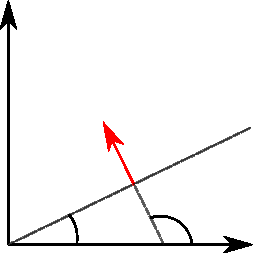
\includegraphics[width=0.4\textwidth]{Figures/SkyrmionAnglesv2}};
\node at (180pt,20pt) {\Large{$x$}};
\node at (20pt,180pt) {\Large{$y$}};
\node at (70pt,23pt) {\Large{$\phi$}};
\node at (140pt,35pt) {\Large{$\Phi$}};
\node at (80pt,110pt) {\textcolor{red}{\Large{$\left(m_x,m_y\right)$}}};
\end{tikzpicture}
\caption{The definitions of the angles $\Phi$ and $\phi$. In this case $\Phi = \phi+\pi/2$, in other words it can be described by $\Phi =m\phi+\psi$ with $m=1$ and $\psi=\pi/2$.}
\label{fig:PhiFig}
\end{figure}
Due to the periodical nature of the angles, $m$ is constrained to be an integer. The phase difference $\psi$ between $\Phi$ and $m\phi$ is a constant called the helicity of the skyrmion. If one plugs in the ansatz \eqref{eq:SkyrmionMVec} into \eqref{eq:SkyrmionNumber}, one finds that
\begin{align}
N_{\textrm{sk}} = \frac{m}{4\pi}\int_0^{2\pi}\d\phi \int_0^{\infty}\d r \sin\theta(r) \frac{\partial\theta(r)}{\partial r} = - \frac{m}{2} \cos(\theta(r))|_{(r = 0)}^{(r=\infty)}.
\end{align}
Unless $m$ is an even number, one must require that $\theta(r = 0) = 0$ and $\theta(r = \infty) = \pi$, or $\theta(r = 0) = \pi$ and $\theta(r = \infty) = 0$ for the skyrmion number to be an integer and not a half-integer.

The skyrmion needs a certain type of physical mechanism in the material to be a stable state. This mechanism will allow a lower energy state by having the neighbouring spins not be entirely parallel to each other, like the symmetric exchange interaction wants them to be. One of these mechanisms is the Dzyaloshinskii--Moriya interaction, which is the stabilizing mechanism of skyrmions we will consider in this thesis. Other mechanisms that can also cause the magnetic skyrmion to be a stable state are long-ranged magnetic dipolar interactions \cite{Lin1973}, frustrated exchange interactions \cite{Okubo2012} and four-spin exchange interactions \cite{Heinze2011}. If we consider the interfacial DMI energy density in \eqref{eq:DMInterface} and plug in our ansatz for the magnetization of the skyrmion, one finds that
\begin{align}
\epsilon_{\text{DM}}^{\textrm{(interface)}} = D\cos((m-1)\phi + \psi)\left(\frac{\partial\theta}{\partial r} + \frac{m}{r}\sin\theta\cos\theta\right).
\end{align}
For the DMI to have a net energy contribution, we must remove the dependence on $\phi$ as the average of a harmonic function over the plane will be zero. We therefore require that $m = 1$, which is not an even number, meaning we must apply the boundary conditions for $\theta(r)$ mentioned earlier. The helicity $\psi$ is then chosen to minimize the energy contribution from DMI, which leaves us with the two options $\psi = 0$ and $\psi = \pi$, depending on the sign of $D$ and the $\theta$ profile. Due to the boundary conditions for $\theta$, the magnetization in the core of the skyrmion points in the opposite direction of the magnetization far away from the skyrmion core. The magnetization direction far away from the core must therefore be a stable direction in the energy. This can be done in a system with an easy axis parallel to that direction. If we consider a skyrmion in a thin film, which makes sense with our choice of interfacial DMI, the easy axis must be perpendicular to that film. In other words, we need a thin-film system with perpendicular magnetic anisotropy. Finally, as our system is ferromagnetic, we also need to include the symmetric exchange interaction. This is also a mechanism that allows us to treat the skyrmion in the micromagnetic model, where we assume that the magnetization can be estimated by a smooth and slowly varying function. This assumption was for example used in the Taylor expansion of the DMI Hamiltonian. Our model then has the energy density given by
\begin{align}
\nonumber \epsilon &= \epsilon_{\text{EX}} + \epsilon_{\text{PMA}} + \epsilon_{\text{DM}}^{\textrm{(interface)}} \\
&=A \left[\left(\frac{\partial\theta}{\partial r}\right)^2 + \frac{\sin^2\theta}{r^2}\right] + K\sin^2\theta + D\cos\psi\left(\frac{\partial\theta}{\partial r} + \frac{\sin\theta\cos\theta}{r}\right),
\end{align}
assuming a magnetization profile given by \eqref{eq:SkyrmionMVec}. The energy is independent of $\phi$ due to our choice of $m$, but it remains a function of $\theta$ and $r$. As the skyrmion is a ground state, we can find the function $\theta(r)$ by minimizing the energy. Using the condition
\begin{align}
\frac{\delta\epsilon(\theta, r)}{\delta\theta(r)} = \frac{\partial\epsilon}{\partial\theta} - \frac{\textrm{d}}{\textrm{d}r} \frac{\partial\epsilon}{\partial (\frac{\partial\theta}{\partial r})} = 0
\end{align}
and introducing the dimensionless length $\tilde{r} = r D/A$, one ends up with the following differential equation for $\theta(r)$:
\begin{align}
\label{eq:ODEtheta}
\frac{\partial^2\theta}{\partial\tilde{r}^2} + \frac{1}{\tilde{r}}\frac{\partial\theta}{\partial\tilde{r}} - \frac{\sin\theta\cos\theta}{\tilde{r}^2}+\cos\psi\frac{\sin^2\theta}{\tilde{r}}-\frac{AK}{D^2}\sin\theta\cos\theta = 0.
\end{align}
Definining the ratio $AK/D^2$ as a parameter $C$, one can solve this equation numerically for a given $C$. Some numerical solutions are shown in Figure \ref{fig:ThetaProfile} when the boundary conditions $\theta(r = 0) = \pi$ and $\theta(r = \infty)$ have been used. It should be noted that this differential equation only has a solution when $\cos\psi = 1$ for the chosen boundary conditions. The solutions for the different helicities $\psi_1 = 0$ and $\psi_2 = \pi$ have a simple relation, however. This relation can be verified to be
\begin{align}
\label{eq:ThetaHelicityRelation}
\theta_{\psi_1}(r) = \pi - \theta_{\psi_2}(r),
\end{align}
as $\cos\psi$ is antisymmetric under a swap in helicities, and $\frac{\partial^2\theta}{\partial\tilde{r}^2}$, $\frac{\partial\theta}{\partial\tilde{r}}$, $\cos\theta_{\psi_i}$ are all antisymmetric under the relation above.
\begin{figure}[h!]
\begin{center}
\begin{tikzpicture}
\node[above right] (img) at (0,0)
{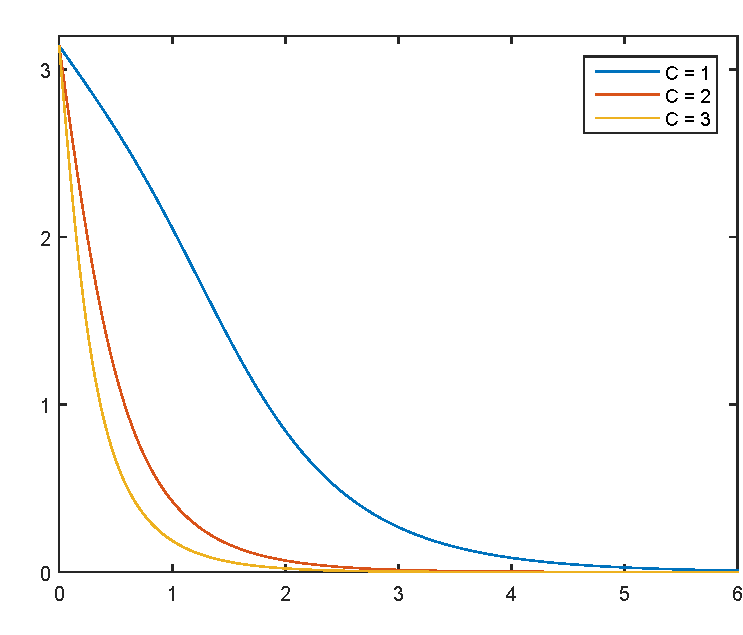
\includegraphics[width=0.6\textwidth]{Figures/SkyrmionRadialProfilesv2.pdf} };
 \node [right=of img,rotate=90,anchor=north,yshift=11cm,xshift=0.2cm] {\Large{$\theta(\tilde{r})$}}; 
 \node at (150pt,8pt) {\Large{$\tilde{r}$}};
\end{tikzpicture}
%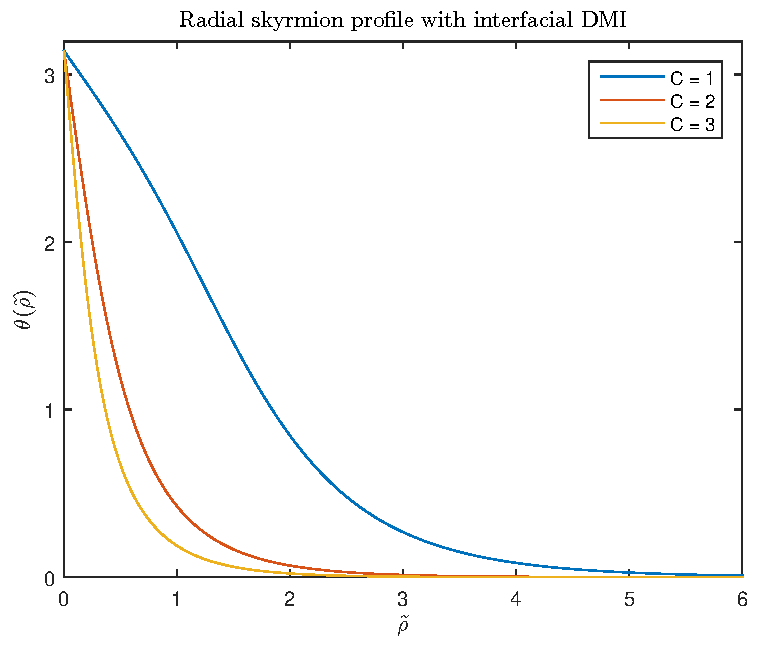
\includegraphics[width=0.6\textwidth]{Figures/SkyrmionRadialProfiles.pdf} 
\caption{The solution of the out-of-plane angle $\theta$ of the skyrmion profile for different values of $C$.}
\label{fig:ThetaProfile} 
\end{center}
\end{figure}
The two different skyrmions for the two different choices in helicities $\psi$ are illustrated in Figure \ref{fig:HedgehogSkyrmions}. This type of skyrmions is called a hedgehog skyrmion, due to the magnetization pattern that curves into or away from the core.
\begin{figure}[h!]
\centering
\begin{subfigure}{.49\textwidth}
  \centering
  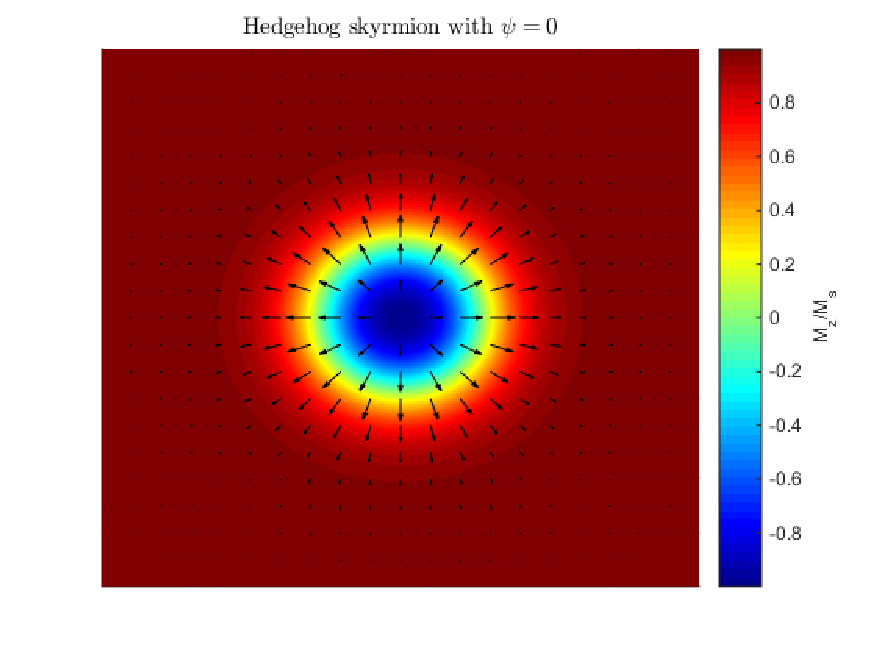
\includegraphics[width=\linewidth]{Figures/HedgehogSkyrmionPsi0.pdf}
  \caption{}
  \label{fig:HedgehogSkyrmion1}
\end{subfigure}
\begin{subfigure}{.49\textwidth}
  \centering
  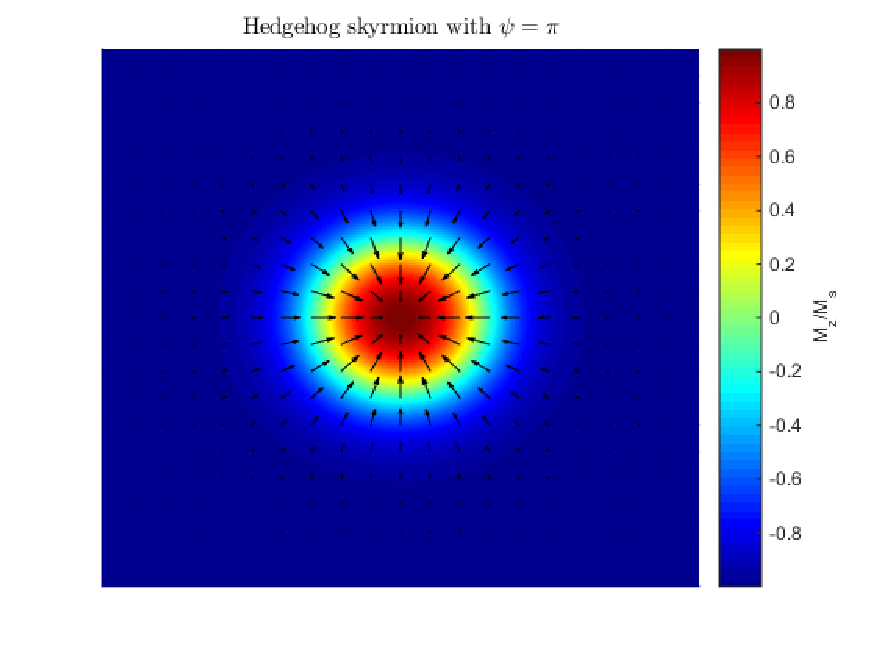
\includegraphics[width=\linewidth]{Figures/HedgehogSkyrmionPsiPi.pdf}
  \caption{}
  \label{fig:HedgehogSkyrmion2}
\end{subfigure}
\newline
\begin{subfigure}{.49\textwidth}
  \centering
  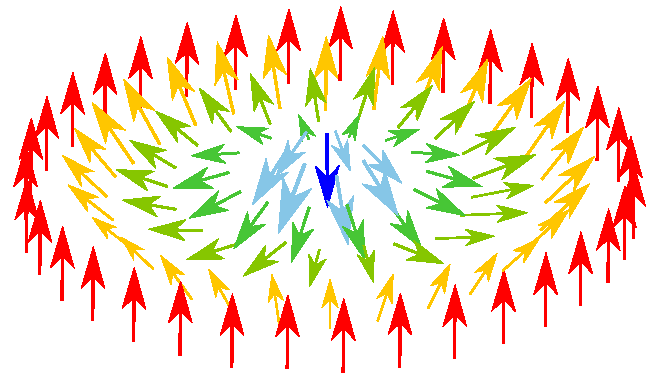
\includegraphics[width=\linewidth]{Figures/HedgehogSkyrmion}
  \caption{}
  \label{fig:HedgehogSkyrmion3}
\end{subfigure}
\caption{A hedgehog skyrmion with a helicity \textbf{(a)} $\psi = 0$ and \textbf{(b)} $\psi = \pi$. The in-plane component of the magnetization is visualized by the vectors, while the $z$-component is shown in the background color. A 3D representation of a hedgehog skyrmion with $\psi = 0$ is shown in \textbf{(c)}, this figure is based on a figure in \cite{EverschorDissertation}.}
\label{fig:HedgehogSkyrmions}
\end{figure}

The results shown so far are based on a system that is stabilized by the interfacial form of DMI. Skyrmions can also be stabilized by the bulk form of DMI, however. Using the ansatz of the skyrmion magnetization profile in \eqref{eq:SkyrmionMVec} in the expression for bulk DMI given by \eqref{eq:DMBulk}, we find the same energy density as for the interfacial DMI $\epsilon_{\text{DM}}^{\textrm{(interface)}}$ with the substitution $\cos\psi \rightarrow \sin\psi$. In other words, the skyrmion stabilized by the bulk DMI will have helicities $\psi=\pm\pi/2$, and the $\theta(r)$ profile will be the same as for the hedgehog skyrmions stabilized by the interfacial DMI. These types of skyrmions are called spiral skyrmions, as the in-plane magnetization either spirals clockwise or counter-clockwise around the core. From now on we will mostly consider hedgehog skyrmions stabilized by the interfacial form of DMI, as that is the form of DMI that is found in layered thin-film systems that we will study.

\section{Symmetries}
Before moving on to the dynamical properties of the skyrmions we will take a brief interlude to discuss the symmetries of the skyrmion and the LLG equation. This will help us to get further insight into how the different terms in the LLG equation work, and how the skyrmion solutions are related to each other.
\subsection{Time reversal}
Time reversal (or T-symmetry) is a transformation where one reverses the time ($t \rightarrow -t$) as the name indicates. Physical laws that are symmetric under time reversal are reversible processes, while physical laws that break the time reversal symmetry are irreversible processes. Physical variables are either even or odd during time reversal. If they are even they are symmetric under time reversal, and if they are odd they are asymmetric during time reversal. To discuss whether the LLG equation breaks time reversal we need to know how the magnetization $\mathbold{M}$ and the magnetic field $\mathbold{H}$ transform (the constants $\alpha$, $M_s$ and $\gamma$ are all even under time reversal, as they are scalars unrelated to the weak force). It turns out that both $\mathbold{M}$ and $\mathbold{H}$ are odd during time reversal \cite{Jackson}. If we then apply the time reversal transformation to the LLG equation, we end up with
\begin{align}
\label{eq:LLG_TR}
\frac{\textrm{d}\mathbold{M}}{\textrm{d}t} = -\gamma\mathbold{M}\times\mathbold{H}-\frac{\alpha}{M_s}\mathbold{M}\times\frac{\textrm{d}\mathbold{M}}{\textrm{d}t}.
\end{align}
Comparing this to the LLG equation in \eqref{eq:LLG} we see that the LLG equation breaks T-symmetry due to the damping term proportional to $\alpha$. The damping is a dissipative motion, and is therefore an irreversible process. The precession of the magnetization around the magnetic field on the other hand does not break T-symmetry, and is therefore a reversible process.

\subsection{Parity and chirality} \label{sec:Parity}
Parity is a transformation operation which changes the sign of all three cartesian coordinates simultaneously ($\mathbold{r}\rightarrow-\mathbold{r}$), in other words it is a point reflection through the origin. 
%In cylindrical coordinates a parity transformation can be written as $r \rightarrow r$, $\phi \rightarrow \phi \pm \pi$, $z \rightarrow -z$. Let us now first consider the parity transformation of a magnetic skyrmion. The skyrmion depends on the cylindrical coordinates $r$ and $\phi$, as seen from \eqref{eq:SkyrmionMVec}. There is no explicit dependence on $z$, meaning the magnetization pattern is isotropic in the $z$-direction. Since $r$ is even under the parity transformation, the entire effect of the operation lies in the change in $\phi$. We remember that the in-plane angle of the magnetization $\Phi$ was given by $\Phi = \phi + \psi$. After a parity transformation this becomes $\Phi = \phi + \psi \pm \pi$. The helicity $\psi$ is a constant, and we can therefore include the change $\pm\pi$ in the helicity of the skyrmion. A magnetic skyrmion has two possible helicities (a hedgehog skyrmion stabilized by interfacial DMI can have $\psi = 0$ or $\psi = \pi$, while a spiral skyrmion stabilized by bulk DMI can have $\psi = \pm\pi/2$) that are a constant $\pi$ apart from each other. A parity transformation then transforms the helicity of the magnetic skyrmion to its other possible value. As a cross-check we also see that two consecutive parity transformations become an identity transformation. In other words, the magnetization pattern of the skyrmion breaks parity. This is a result of the Dzyaloshinskii--Moriya interaction, which is an interaction that violates parity. 
To dicuss parity we first introduce the notion of pseudovectors and pseudoscalars. Normally, vectors are odd under a parity transformation, meaning the transformation changes the sign of the vector, while scalars are even under a parity transformation. Pseudovectors and pseudoscalars behave the opposite way, however. A pseudovector will behave as a vector during a rotation, but during a reflection it behaves differently. An example of a pseudovector is the antisymmetric cross-product between two vectors, which is illustrated in Figure \ref{fig:Parity}. 
\begin{figure}[h!]
\centering
\begin{subfigure}{.43\textwidth}
  \centering
    \begin{tikzpicture}
\node[above right] (img) at (0,0) {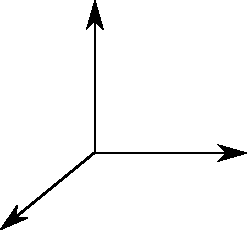
\includegraphics[width=1\textwidth]{Figures/Cartesianv2}};
\node at (40pt,15pt) {\Large{$\mathbold{\hat{x}}$}};
\node at (95pt,175pt) {\Large{$\mathbold{\hat{z}}$}};
\node at (190pt,85pt) {\Large{$\mathbold{\hat{y}}$}};
\end{tikzpicture}
  \caption{}
\end{subfigure}%
\hspace{1cm}
\begin{subfigure}{.33\textwidth}
  \centering
    \begin{tikzpicture}
\node[above right] (img) at (0,0) {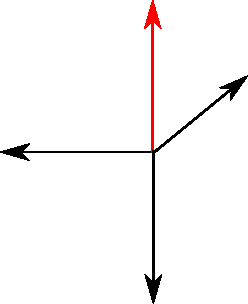
\includegraphics[width=1\textwidth]{Figures/Parityv2}};
\node at (10pt,80pt) {\Large{$\mathbold{\hat{y}}'$}};
\node at (80pt,15pt) {\Large{$\mathbold{\hat{z}}'$}};
\node at (150pt,150pt) {\Large{$\mathbold{\hat{x}}'$}};
\node at (60pt,175pt) {\textcolor{red}{\Large{$\mathbold{\hat{x}}'\times\mathbold{\hat{y}}'$}}};
\end{tikzpicture}
  \caption{}
\end{subfigure}
\caption{An illustration of how cross-products do not transform as vectors under parity. In \textbf{(a)} we see a cartesian coordinate system. Performing a parity transformation on this right-handed coordinate system gives us the left-handed coordinate system in \textbf{(b)}. The pseudovector $\mathbold{\hat{x}}\times\mathbold{\hat{y}}$, which in our right-handed system is equal to $\mathbold{\hat{z}}$, is even under the parity transformation, while the vector $\mathbold{\hat{z}}$ is odd. }
\label{fig:Parity}
\end{figure}
A pseudoscalar is the symmetric dot-product between a pseudovector and a vector. When studying the parity of an expression, the folowing relations may be useful:
\begin{subequations}
\begin{align}
    \label{eq:Pseudovector}
    \textrm{vector}\times\textrm{vector} &= \textrm{pseudovector}, \\
    \label{eq:Vector}
    \textrm{vector}\times\textrm{pseudovector} &= \textrm{vector}, \\
    \label{eq:PseudovectorPseudo}
    \textrm{pseudovector}\times\textrm{pseudovector} &= \textrm{pseudovector}, \\
    \label{eq:Scalar}
    \textrm{vector}\cdot\textrm{vector} &= \textrm{scalar}, \\
    \label{eq:Pseudoscalar}
    \textrm{vector}\cdot\textrm{pseudovector} &= \textrm{pseudoscalar}, \\
    \label{eq:ScalarPseudo}
    \textrm{pseudovector}\cdot\textrm{pseudovector} &= \textrm{scalar}.
\end{align}
\end{subequations}
Now we must consider how the vectors in our equations transform under a parity operation. The relevant vectors are $\mathbold{M}$, $\mathbold{H}$, $\mathbold{E}$, $\mathbold{\nabla}$, $\mathbold{\hat{x}}$, $\mathbold{\hat{y}}$ and $\mathbold{\hat{z}}$. The magnetization and magnetic field are both pseudovectors, and are even under a parity transformation \cite{Jackson}. The unit vectors in cartesian coordinates are ordinary vectors, and therefore odd under a parity transformation. As a consequence, the components of the magnetization $M_x$, $M_y$ and $M_z$ are all pseudoscalars, which can be seen from \eqref{eq:Pseudoscalar}. The electric field is also odd under a parity transformation \cite{Jackson}, which means that the electric field components behave as scalars, as seen from \eqref{eq:Scalar}. Lastly the $\mathbold{\nabla}$ operator also transforms as a vector, and is therefore odd under parity.

We now have all the results we need to consider the parity of the LLG equation, the effective field, the micromagnetic energy and the skyrmion magnetization. Starting off with the LLG equation \eqref{eq:LLG}, we see that it does not break parity explicitly as long as $\mathbold{H}$ is even under a parity transformation by using the relation in \eqref{eq:PseudovectorPseudo}. When considering the micromagnetic energy terms, all are found to be even under a parity transformation with the exception of the DMI terms (which holds true for both the bulk form of DMI in \eqref{eq:DMBulk} and the interfacial form in \eqref{eq:DMInterface}). At first glance, however, it may seem like the interfacial form of the DMI energy density in \eqref{eq:DMInterface} is even under parity. The reason for this is that while going from the original expression in \eqref{eq:DMIHamiltonian} (which is seen to break parity from \eqref{eq:PseudovectorPseudo} as $\mathbold{D}_{ij}$ is a vector and $\mathbold{S} \propto \mathbold{M}$ is a pseudovector) we have eliminated a cross product. As one can see in \eqref{eq:DMInterfaceCrossP} we have terms that go as $\mathbold{\hat{x}}\cdot(\mathbold{\hat{y}}\times\mathbold{\hat{z}})$ and $\mathbold{\hat{y}}\cdot(\mathbold{\hat{z}}\times\mathbold{\hat{x}})$. In \eqref{eq:DMInterface} these vector expressions are simplified to be unity, which is correct, but hides some of the information when we want to study parity. As $\mathbold{\hat{y}}\times\mathbold{\hat{z}}$ and $\mathbold{\hat{z}}\times\mathbold{\hat{x}}$ are pseudovectors, $\mathbold{\hat{x}}\cdot(\mathbold{\hat{y}}\times\mathbold{\hat{z}})$ and $\mathbold{\hat{y}}\cdot(\mathbold{\hat{z}}\times\mathbold{\hat{x}})$ are in fact pseudoscalars which we can see from \eqref{eq:Pseudoscalar}. So in reality there is a unity pseudoscalar lurking in the expression in \eqref{eq:DMInterface}, making it seem like it is even under parity while in reality it is not. This same pseudoscalar is carried onwards to the DMI term in the effective field in \eqref{eq:EffectiveField}, making part of the effective field odd under parity and thereby violating parity in the LLG equation.

%In summary, it is found that the Dzyaloshinskii--Moriya interaction is the cause of the parity violation in the LLG equation and the skyrmion magnetization pattern, regardless if it is in its bulk or interfacial form.

Moving on to the skyrmion magnetization pattern we use that $\mathbold{M}$ is even under parity, while its components $M_x$, $M_y$ and $M_z$ are not. Remembering that $\mathbold{\hat{M}} = \left(\cos\Phi\sin\theta, \sin\Phi\sin\theta, \cos\theta\right)$ we see that all the components are odd under parity if $\Phi$ transforms as $\Phi \rightarrow \Phi \pm \pi$ and $\theta$ transforms as $\theta\rightarrow\pi-\theta$. This is reminiscent of something we have seen earlier. In Section \ref{sec:Skyrmions} we noted that the solutions for the two different helicities were related by \eqref{eq:ThetaHelicityRelation}, which is the same as the way $\theta$ transforms under parity. In addition, the two possible helicities for the individual types of skyrmions (hedgehog or spiral) are always a phase $\pm\pi$ apart. The term $\pm\pi$ in the transformation of $\Phi$ under parity can then be included in the helicity, meaning the parity transformation changes the helicity of the skyrmion. The two possible solutions of the skyrmions, such as the hedgehog skyrmions in Figure \ref{fig:HedgehogSkyrmion1} and \ref{fig:HedgehogSkyrmion2}, are therefore related to each other via parity. If the skyrmion in \ref{fig:HedgehogSkyrmion1} is the solution in a right-handed coordinate system, the skyrmion in \ref{fig:HedgehogSkyrmion2} is the same solution in a left-handed coordinate system, and vice versa.
\begin{figure}[h!]
\centering
\begin{subfigure}{.39\textwidth}
  \centering
  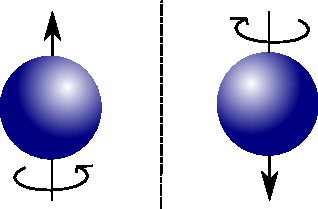
\includegraphics[width=1.0\linewidth]{Figures/UpDownSpinMirror}
  \caption{}
\end{subfigure}%
\hspace{1cm}
\begin{subfigure}{.5\textwidth}
  \centering
  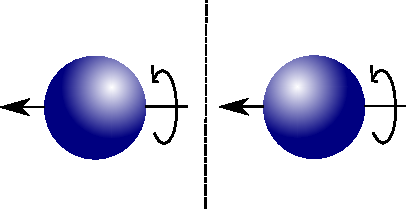
\includegraphics[width=1.0\linewidth]{Figures/LeftSpinMirror}
  \caption{}
\end{subfigure}
\caption{An electron that has a spin vector parallel to a mirror plane will have its spin reversed in its mirror image, as shown in \textbf{(a)}. An electron with a spin perpendicular to the mirror plane, however, will have the same spin as its mirror image as shown in \textbf{(b)}.}
\label{fig:SpinMirror}
\end{figure}
\begin{figure}[h!]
\centering
\begin{subfigure}{.95\textwidth}
  \centering
  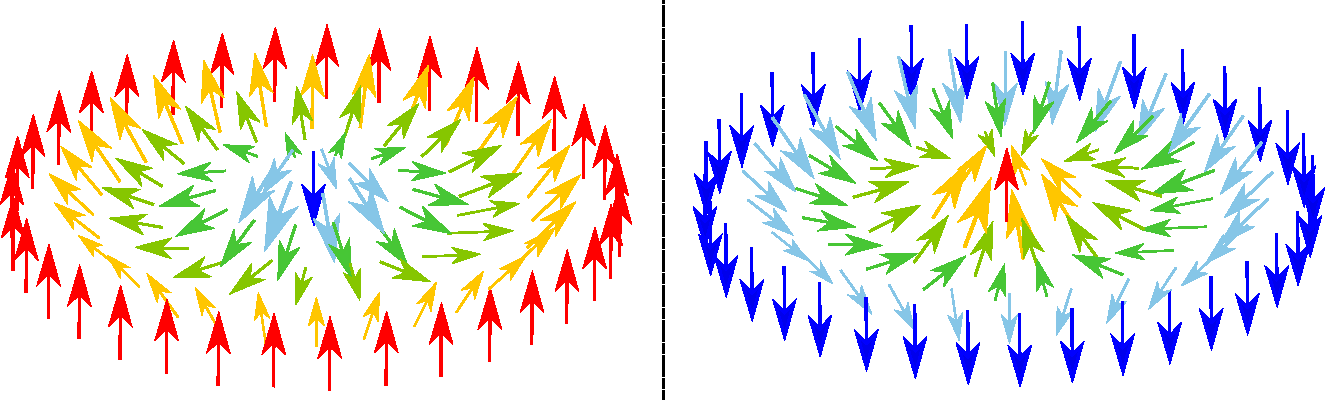
\includegraphics[width=\linewidth]{Figures/MirroredHedgehogSkyrmion.pdf}
  \caption{}
  \label{fig:MirrorHedgehog}
\end{subfigure}

\begin{subfigure}{.95\textwidth}
  \centering
  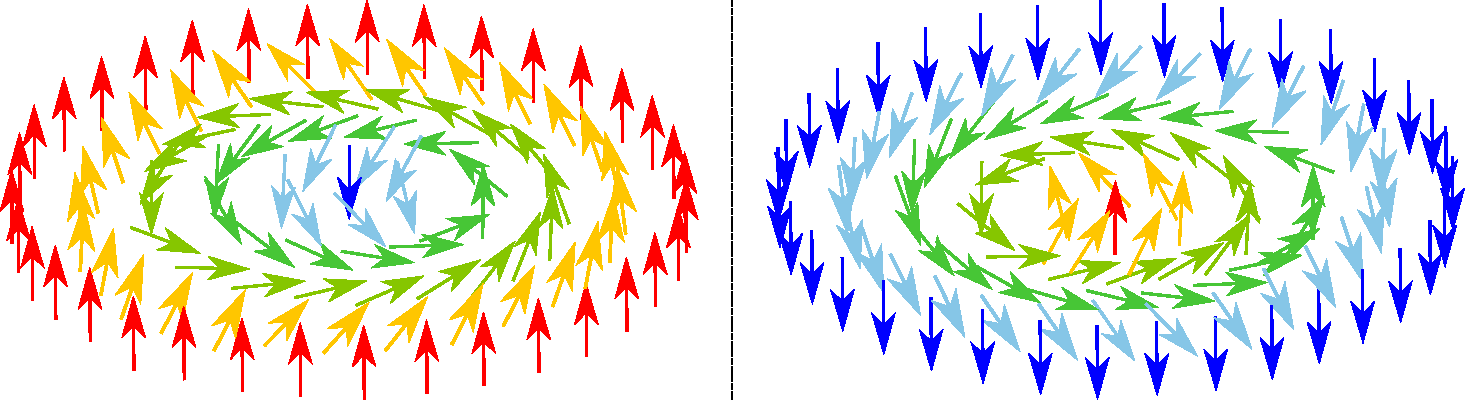
\includegraphics[width=\linewidth]{Figures/MirroredSpiralSkyrmionv2.pdf}
  \caption{}
  \label{fig:MirrorSpiral}
\end{subfigure}
\caption{The mirror images of \textbf{(a)} a hedgehog skyrmion, and \textbf{(b)} a spiral skyrmion. The mirror images can not be aligned with the original image, and the skyrmions are therefore chiral objects. The skyrmion figures are based on the figures in \cite{EverschorDissertation}.}
\label{fig:ChiralitySkyrmions}
\end{figure}

As a final comment on the symmetries of the skyrmions, we want to discuss their chirality. An object is defined to be chiral if its mirror image or reflection is impossible to align with the original object. The most common example of chirality is hands. When holding your right hand in front of a mirror, the image you see in the mirror is that of a left hand. Obviously, a right hand and a left hand are distinct, and can therefore not be aligned with each other. Hands are then chiral objects. When we are considering a mirror image of a skyrmion, we need to be careful regarding what we take the mirror image of. The mirror image of a skyrmion is \textit{not} the mirror image of the skyrmion magnetization vector field. The magnetization of the skyrmion stems from the average magnetic moment inside a small volume, and the magnetic moment is proportional to the spinning of the electron. As we see in Figure \ref{fig:SpinMirror}, when we mirror the spinning motion of the electron the spin vector is not its mirror image. The component of the spin vector parallel to the mirror plane is flipped, while the perpendicular component is the same for both the original electron and its mirror image. This type of behavior occurs for the mirror image of pseudovectors (also known as axial vectors). As the magnetization is also a pseudovector, the mirror images of the skyrmion profiles will behave in the same manner, and are as shown in Figure \ref{fig:ChiralitySkyrmions}. No matter how one rotates the mirror images of the skyrmion magnetization, one can not align them with the original skyrmion. The skyrmions are therefore chiral. This is a consequence of the broken parity of the skyrmion magnetization profile due to the Dzyaloshinskii--Moriya interaction. If the parity transformation of an object is not an identity transformation, it is a chiral object.

\section{The Thiele equation}
In the special case of a time-dependent magnetization pattern that can be written as $\mathbold{M}(\mathbold{r}-\mathbold{R}(t))$, Thiele recognized \cite{Thiele1973} that the time derivative can be written as 
\begin{align}
\label{eq:ThieleRelation}
\frac{\textrm{d} \mathbold{M}}{\textrm{d} t} = \frac{\partial \mathbold{R}}{\partial t}\frac{\partial \mathbold{M}}{\partial \mathbold{R}} = \frac{\partial \mathbold{R}}{\partial t} (-\frac{\partial \mathbold{M}}{\partial \mathbold{r}}) = -(\mathbold{v}\cdot\nabla)\mathbold{M}.
\end{align}
The form $\mathbold{M}(\mathbold{r}-\mathbold{R}(t))$ indicates that the magnetization pattern performs a translation without deformation of the original magnetization profile. Once the equilibrium profile at some time $t_0$ is known, the motion of the entire magnetization pattern can be described by the time-dependent position of some distinct part of the magnetization pattern, like the skyrmion core. If one replaces all time derivatives with Thiele's relation as given above in the LLG equation, one can rewrite the LLG equation to the Thiele equation (as shown by Kr\"{u}ger in \cite{krugerDissertation}):
\begin{align}
\label{eq:Thiele}
\mathbold{F} + \mathbold{G}\times(\mathbold{v}+b_J\mathbold{\hat{j}}_e) - D(\alpha\mathbold{v}+\beta b_J\mathbold{\hat{j}}_e) = 0.
\end{align}
This is a force equation with the definitions
\begin{subequations}
\label{eq:ThieleFGD}
\begin{align}
\label{eq:ThieleF}
\mathbold{F} &= -\frac{\partial E}{\partial \mathbold{R}} = -\mu_0\int \d V\sum_k (\mathbold{\nabla}M_k)(H_k), \\
\label{eq:ThieleG}
\mathbold{G} &= \frac{2\pi M_s\mu_0 d}{\gamma'}\left[\cos\theta\right]_{\theta(r=0)}^{\theta(r=\infty)} \mathbold{\hat{z}},\\
\label{eq:ThieleD}
D &= \frac{\pi M_s \mu_0 d}{\gamma '} \int_0^{\infty} \d r \left(r\left(\frac{\partial \theta}{\partial r}\right)^2+\frac{\sin^2\theta}{r}\right),
\end{align}
\end{subequations}
where $d$ is the thickness of the film. The vector $\mathbold{F}$ is a force originating from an inhomogenous energy landscape or a magnetic field that is not parallel to the local magnetization (in other words a field not aligned with the effective field). $\mathbold{G}$ is a gyrovector that only depends on the direction of the magnetization in the skyrmion core and far away from the core. The force in the Thiele equation that is dependent on $\mathbold{G}$ is often called the Magnus force, and is a counter force to the Lorentz forces from emergent electromagnetic fields around the skyrmion \cite{Everschor-Sitte2014}, which we will discuss in the next section. Lastly, $D$ denotes the strength of a dissipative force that moves the skyrmion in the direction of the electron flow and it is dependent on the radial profile of the out-of-plane angle $\theta$ of the skyrmion. An illustration of the force balance in the Thiele equation is shown in Figure \ref{fig:Thiele}. The Thiele equation is less rigid than the LLG equation due to the ansatz that there is an absence of deformation of the skyrmion, but in the case of a pure translational motion of the skyrmion the Thiele and LLG equations are entirely equivalent.
\begin{figure}[h!]
\centering
  \centering
    \begin{tikzpicture}
\node[above right] (img) at (0,0) {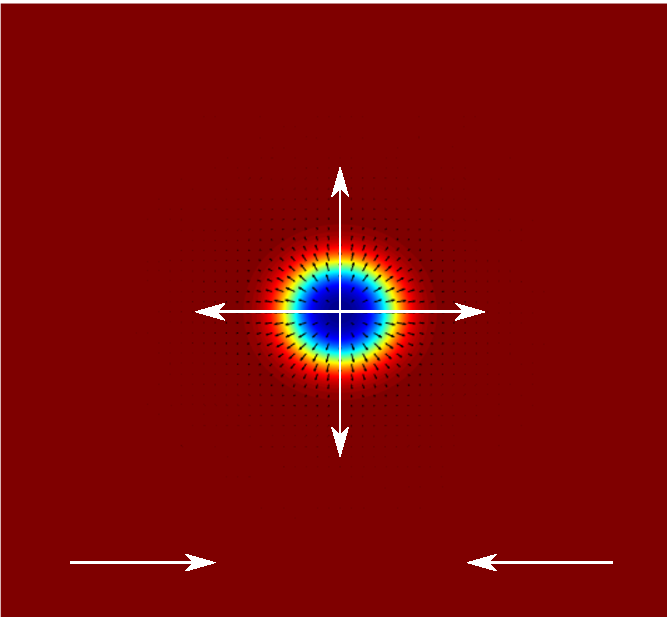
\includegraphics[width=0.6\textwidth]{Figures/SkyrmionThielev2}};
\node at (60pt,40pt) {\textcolor{white}{\Large{$\mathbold{\hat{j}}$}}};
\node at (230pt,40pt) {\textcolor{white}{\Large{$\mathbold{v}$}}};
\node at (50pt,130pt) {\textcolor{white}{\Large{$-D\beta b_J\mathbold{\hat{j}}$}}};
\node at (230pt,130pt) {\textcolor{white}{\Large{$-D\alpha \mathbold{v}$}}};
\node at (140pt,60pt) {\textcolor{white}{\Large{$\mathbold{G}\times \mathbold{v}$}}};
\node at (147pt,200pt) {\textcolor{white}{\Large{$\mathbold{G}\times b_J\mathbold{\hat{j}}$}}};
\end{tikzpicture}
\caption{An example of the forces in the Thiele equation. In the example shown $\alpha=\beta$ and $\mathbold{v}=-b_J\mathbold{\hat{j}}$. The force vectors are only there to show direction, and not magnitude. The goal of the Thiele equation is finding a velocity $\mathbold{v}$ that makes all the forces add up to zero.}
\label{fig:Thiele}
\end{figure}

\section{Berry phase, emergent fields, and the topological Hall effect} \label{sec:Berry}
When discussing the dynamics of skyrmions, it will be useful to have some knowledge on Berry phases. The Berry phase \cite{Berry1984}, also known as a geometric phase, is a rotational angle gained by a vector when it undergoes parallel transport on a closed path on a curved surface, as illustrated in Figure \ref{fig:Berry}.
\begin{figure}[h!]
\centering
  \centering
  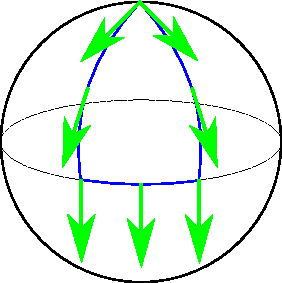
\includegraphics[width=.4\linewidth]{Figures/BerryPhase}
\caption{When a vector undergoes a parallel transport along a closed path on a sphere, it will not be in the same state when arriving back at its starting point. It is rotated with respect to the initial vector, and this rotational angle is known as the Berry phase.}
\label{fig:Berry}
\end{figure}
If the closed path was in a plane, however, the vector will not gain a rotation along its cycle. Skyrmions are magnetization patterns that can be located in a plane, so why is then the Berry phase of interest when electrons move in that plane? When we first started discussing skyrmions, we said that the skyrmion wraps around the unit sphere. In other words, while the magnetization of the skyrmion is located in a plane, the topology of the magnetization pattern behaves in a way so that it can be described as lying on a spherical surface \cite{Everschor-Sitte2014}. 
\begin{figure}[h!]
\centering
\begin{subfigure}{.5\textwidth}
  \centering
  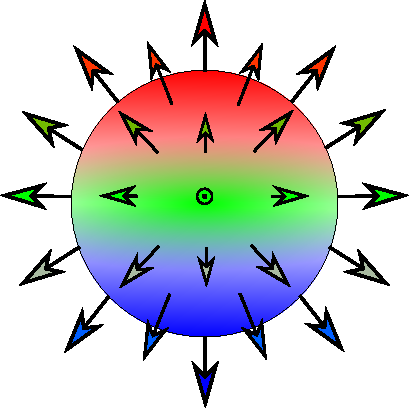
\includegraphics[width=1.0\linewidth]{Figures/HedgehogSphere}
  \caption{}
\end{subfigure}%
\hspace{1cm}
\begin{subfigure}{.35\textwidth}
  \centering
  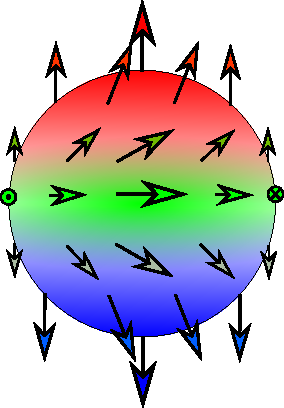
\includegraphics[width=1.0\linewidth]{Figures/SpiralSphere}
  \caption{}
\end{subfigure}
\caption{Skyrmions magnetization patterns mapped onto a spherical surface. The magnetization at $r=0$ is at the bottom of the sphere, while the magnetization at $r=\infty$ is at the top. In \textbf{(a)} we see a hedgehog skyrmion with $\psi = 0$, while in \textbf{(b)} we see a spiral skyrmion with $\psi = \pi/2$.}
\label{fig:SkyrmionSphere}
\end{figure}
This is illustrated in Figure \ref{fig:SkyrmionSphere}. So despite the fact that the conduction electrons from an applied current are moving in a plane, their magnetic moment will still gain a Berry phase when following the magnetization of the skyrmion adiabatically due to the topology of the skyrmion \cite{Tatara2007, Binz2008}. When moving through the skyrmion magnetization, the conduction electrons path is then bent away from the initial direction of the current. This can be seen as a force acting on the conduction electrons, and then there must be an equal force acting in the opposite direction on the skyrmion magnetization. This movement perpendicular to the current direction is known as the topological Hall effect \cite{Ye1999}, as it depends entirely on the topology of the magnetization.

In magnetization dynamics the Berry phase is most commonly considered through the use of emergent electromagnetic fields. The Berry phase can be found by integrating a quantity known as the Berry vector potential along the closed path in consideration. This vector potential is similar to the vector potential $\mathbold{A}$ in electromagnetism, and the curl of this vector potential (known as the Berry curvature) will then behave as a magnetic field \cite{kanazawa2015charge}. This emergent magnetic field, which is associated with the topology of the magnetization and not its magnetic flux, is given by \cite{Nagaosa2012, Schulz2012}
\begin{align}
    \mathbold{B}_i^e = \frac{\hbar}{2e}\varepsilon_{ijk}\mathbold{\hat{M}}\cdot(\partial_j\mathbold{\hat{M}}\times \partial_k \mathbold{\hat{M}}).
\end{align}
This total magnetic flux from this emergent field is quantized by the skyrmion number $N_{\textrm{sk}}$ given by \eqref{eq:SkyrmionNumber}, which can be seen by integrating the expression above over the skyrmion plane. This emergent magnetic field then causes the conduction electrons to experience a Lorentz force
\begin{align}
    \mathbold{F}_{\textrm{Lorentz}} = q(\mathbold{E} + \mathbold{v}\times\mathbold{B}).
\end{align}
If one assumes the skyrmion magnetization to be localized in the $xy$-plane and to be isotropic in the $z$-direction, then the emergent field $\mathbold{B}_i^e$ points along the $z$-axis. This means that the Lorentz force originating from the emergent magnetic field is localized in the $xy$-plane, and is perpendicular to the motion of the conduction electrons. This bending of the electrons' motion can induce a motion of the skyrmion perpendicular to the direction of the current. In addition to the emergent magnetic field, there will also be an emergent electric field once the skyrmion magnetization starts moving, for example due to spin-transfer torques where the magnetic moment of the conduction electrons is transferred to the local magnetization. As seen from the Maxwell--Faraday equation,
\begin{align}
    \nabla\times\mathbold{E} = -\partial_t\mathbold{B},
\end{align}
once the magnetization pattern starts moving the emergent magnetic field will become time dependent, and thereby induce an emergent electric field. This emergent field is given by
\begin{align}
\label{eq:EmergentE}
\mathbold{E}_i^e = \frac{\hbar}{e} \mathbold{\hat{M}}\cdot(\partial_i\mathbold{\hat{M}}\times\partial_t\mathbold{\hat{M}}).
\end{align}
This electric field will also cause the electrons to feel a Lorentz force, and as we can see from the expression above this force is perpendicular to the motion of the skyrmion. Through these emergent fields we can then get an intuitive explanation of the topological Hall effect.

We have now discussed qualitatively the dynamics of the skyrmion, and why its dynamics distinguishes itself from topologically trivial magnetization patterns. Building upon this discussion, we will in the next chapter start studying the dynamics of the skyrmion more quantitatively by both analytical and numerical calculations.